\chapter{Grundlagen}
\label{chap:grundlagen}
Container werden häufig als leichtgewichtige \glspl{acr-vm} beschrieben. Dies ist allerdings nicht  richtig. Wie in \fref{fig:containerVsVm} zu erkennen, virtualisieren Container kein vollständiges \gls{acr-os}, sondern lediglich das benötigte Dateisystem. Dabei wird der Kernel des Hosts nicht virtualisiert, sondern mitverwendet. Dies macht Container deutlich leichtgewichtiger als \glspl{acr-vm}, isoliert allerdings weniger umfangreich als diese.
\begin{figure}[h]
		\subfigure[Container]{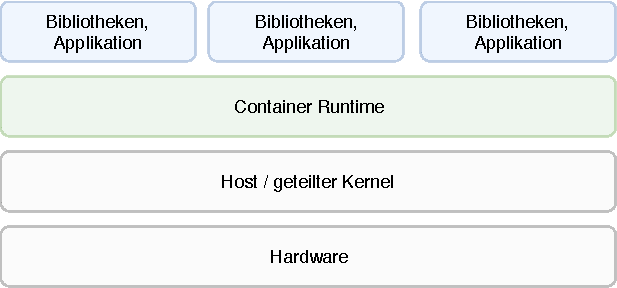
\includegraphics[width=0.49\textwidth]{bilder/container-stack-isolation.pdf}}
		\hfill
		\subfigure[\glspl{acr-vm}]{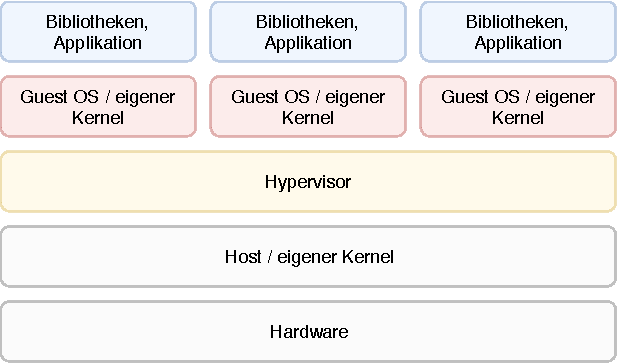
\includegraphics[width=0.49\textwidth]{bilder/vm-stack-virtualisation.pdf}}
		\caption{Container Isolation im Vergleich zu \glspl{acr-vm}}
		\label{fig:containerVsVm}
\end{figure}

Dieses Kapitel behandelt alle benötigten Grundlagen, die zur Isolation eines Prozesses benötigt werden. Es werden vorhandene Standards wie die \gls{acr-oci} und benötigte Systemcalls wie \gls{acr-chroot} näher erläutert. Zudem wird beschrieben, wie die Isolation, die Container bieten, durch Systemmittel des Linux-Kernels selber erreicht wird.

\section{Standards}
\label{sec:standards}
Durch die immer größere Verwendung von Containern und die Verbreitung verschiedener Container-Runtimes ist die Standardisierung eine wichtige Aufgabe. Folgend werden Standardisierungsprojekte aufgezählt, die bestehenden Spezifikationen erläutert und aktuelle Aufgaben der Projekte näher betrachtet.
\subsection{App Container}
\label{sec:appc}
\Gls{acr-appc} ist ein Standard, der viele Aspekte innerhalb der Con"-tainer-Landschaft behandelt. Dabei lag die Hauptaufgabe darin, eine Laufzeitumgebung, wie auch das \gls{gls-image}-Format und die Verbreitung von \glspl{gls-image} zu standardisieren. Seit 2016 wird das Projekt nicht mehr aktiv weiterentwickelt, da mit der Gründung der \gls{acr-oci} ein größeres Standardisierungsprojekt entstand. Bestandteile der \gls{acr-appc} wurden von der \gls{acr-oci} übernommen und dienen als Vorlage für die Spezifikation dieser.

\subsection{Open Container Initiative}
\label{sec:oci}
Die \gls{acr-oci} ist eine Initiative, die seit 2015 unter der Linux Foundation agiert. Das Ziel der OCI ist es, einen offenen Standard für Container zu schaffen, sodass die Wahl der Container-Runtime nicht mehr zu Inkompatibilität führt. Dabei liegt der Fokus auf eine einfache, schlanke Implementierung \citep{OpenContainerInitiative}. 

Die OCI arbeitet aktuell an drei Spezifikationen. Die runtime-spec standardisiert die Laufzeitumgebung  von Containern. Dabei wird festgelegt, welche Konfiguration, Prinzipien und Schnittstellen Laufzeitumgebungen stellen müssen. Um die Umsetzung der runtime-spec zu fördern, stellt die OCI eine beispielhafte Implementierung durch runC. Das zweite Projekt der OCI ist die image-spec. Dieses versucht einen Standard für \glspl{gls-image} zu definieren. Dabei plant die OCI nicht, vorhandene Image-Formate zu ersetzen, sondern auf diesen aufzubauen und sie zu erweitern \citep{OpenContainerInitiative}.

Wie in \fref{tab:ociVSappc} zu sehen, wurden einige Konzepte des \gls{acr-appc}-Projekts in die \gls{acr-oci} übernommen. Vor allem die \gls{gls-image}-Spezifikation wurde durch die Mitarbeit ehemaliger \gls{acr-appc}-Maintainer gefördert. Seit Mai 2018 publiziert die OCI auch eine Spezifikation zur Verbreitung von Images, die auf der Docker Registry HTTP API basiert. Themen, die außerhalb des Scopes der OCI liegen, werden teilweise in die \gls{acr-cncf} aufgenommen \citep{MakingSenseofContainerStandardsandFoundations:OCICNCFAppcandRkt}.

\begin{table}[h]
	\begin{center}
		\begin{tabu} to 0.9\textwidth{@{}lX[1,c]X[1,c]X[6,l]X[6,r]@{}}
			\toprule
			& \multicolumn{2}{c}{Standard} & \multicolumn{2}{c}{Container Runtime}\\
			\cmidrule{2-5}
			& OCI		& appc		& Docker			& rkt					\\
			\midrule
			Container Image			& \faTimes	& \faCheck	& OCI image-spec 	& App Container Image	\\
			Image Verbreitung		& \faCheck 	& \faCheck	& Docker Registry	& appc Discovery Spec 	\\
			Lokales Speicherformat	& \faCheck	& \faTimes	& keine Spezifikation& keine Spezifikation	\\
			\midrule
			Runtime					& \faCheck	& \faCheck	& runC 				& appc runtime Spec		\\
			\bottomrule
		\end{tabu}
	\end{center}
	\caption{Standards OCI und AppC im Vergleich \citep{MakingSenseofContainerStandardsandFoundations:OCICNCFAppcandRkt}}
	\label{tab:ociVSappc}
\end{table}


\subsection{Cloud Native Computing Foundation}
\label{sec:cncf}
Die \gls{acr-cncf} beschäftigt sich im Gegensatz zur \gls{acr-oci} nicht nur mit Containern, sondern der kompletten \gls{gls-cn}-Landschaft \citep{CNCFCloudNativeInteractiveLandscape}. Projekte wie \gls{acr-k8} und Prometheus werden durch die \gls{acr-cncf} weiterentwickelt und publiziert. Da der Cloud-Native Entwicklungsprozess von Containern getragen wird, spielen Technologien wie containerd und rkt eine entscheidende Rolle für die \gls{acr-cncf} und sind ein großer Teil der \gls{gls-cn}-Landscape, wie in \fref{fig:cncfContainerLandscape} gezeigt. Neben Container-Runtimes beinhaltet die \gls{acr-cncf} auch Projekte zur Orchestrierung von Containern. Außerdem Spezifikationen wie TUF, die das updaten von Software spezifiziert \citep{CloudNativeComputingFoundation}.

\begin{figure}[H]
	\begin{center}
		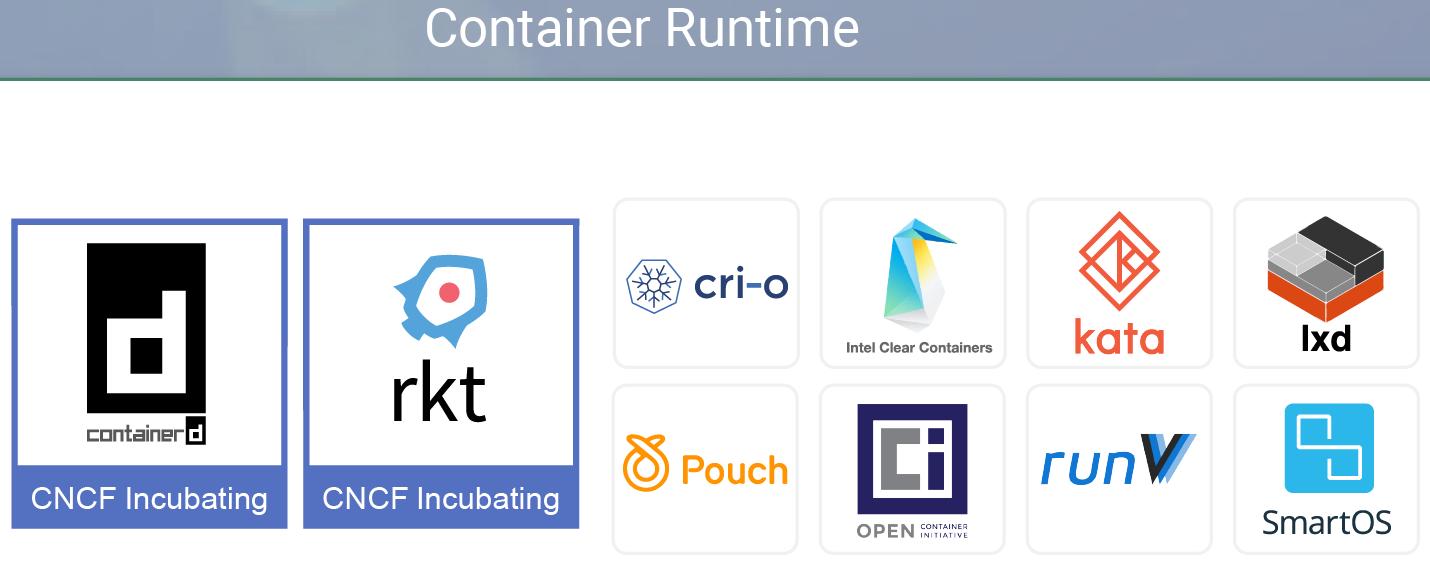
\includegraphics[scale=0.3]{bilder/cncf-container-landscape.png}
		\caption{CNCF Container Runtime Landschaft \citep{CNCFCloudNativeInteractiveLandscape}}
		\label{fig:cncfContainerLandscape}
	\end{center}
\end{figure} 

\section{Funktionsweise}
\label{sec:funktionsweise}

Container isolieren einzelne Prozesse durch verschiedene Kernel-Technologien, die im Folgenden erklärt werden.
\subsection{Change Root}
\label{sec:chroot}
\Gls{acr-chroot} ist ein Unix Systemaufruf, der es erlaubt, einen Prozess in einem anderen Wurzelverzeichnis auszuführen \citep{Chroot1LinuxManualPage}. Daraus folgt, dass der Prozess in einer eigenen Verzeichnisstruktur arbeitet und keine Dateien des Host-\gls{acr-os} ändern kann. \Gls{acr-chroot} erlaubt somit die Isolierung des Dateisystems, die Container nutzen.

\subsection{Control Groups}
\label{sec:cgroups}
\Glspl{acr-cgroup} dienen dazu, Systemressourcen für einzelne Prozesse zu limitieren. Im \gls{acr-os} sind \glspl{acr-cgroup} als Dateihierarchie repräsentiert. Das gesamte \gls{acr-cgroup}-Dateisystem ist unter \texttt{/sys/fs/cgroup/} zu finden. \Glspl{acr-cgroup} stellen zur Steuerung verschiedene Controller zur Verfügung, wie in \fref{tab:cgroupController} zu sehen.

\begin{table}[H]
	\begin{center}
		\begin{tabu} to 0.9\textwidth{@{}lX[2,l]@{}}
			\toprule
			Controller  & Ressource                                                         \\ \midrule
			io          & Zugriff und Nutzung von Block Geräten wie Festplatten             \\
			memory      & Monitoring und Beschränken des Arbeitsspeichers                   \\
			pids        & Limitierung der Anzahl an Unterprozessen                          \\
			perf\_event & Erlaubt Performance Monitoring der Prozesse                       \\
			rdma        & Zugriffe über Remote Direct Memory Access limitieren oder sperren \\
			cpu         & CPU-Zyklen und maximale CPU-Bandwidth                             \\ \bottomrule
		\end{tabu}
		\caption{\Glspl{acr-cgroup}-Controller und deren Verwendung \citep{Cgroups7LinuxManualPage}}
		\label{tab:cgroupController}
	\end{center}
\end{table}

\subsection{Namespaces}
\label{sec:namespaces}
Namespaces abstrahieren einzelne Bereiche des \gls{acr-os}. Sie werden genutzt, um globale Ressourcen zu virtualisieren. Ein Namespace kapselt dabei einzelne Ressourcen (siehe \fref{tab:namespaces}). Veränderungen an diesen sind für alle Prozesse innerhalb desselben Namespaces sichtbar, allerdings außerhalb dieses unsichtbar \citep{Namespaces7LinuxManualPage}.

\begin{table}[h]
	\begin{center}
		\begin{tabu} to 0.9\textwidth{@{}lX[2,l]@{}}
			\toprule
			Namespace			& Ressource				 				\\
			\midrule
			\Gls{acr-cgroup}	& \Gls{acr-cgroup}-Dateisystem 			\\
			IPC					& System V IPC, POSIX Nachrichten 		\\
			Network				& Netzwerk Geräte, Stacks, Ports, ...	\\
			Mount				& Mount Punkte							\\
			PID					& Prozess IDs							\\
			User				& Nutzer und Gruppen IDs				\\
			UTS					& Hostnamen und Domänennamen			\\
			\bottomrule
		\end{tabu}
	\end{center}
	\caption{Linux Namespaces und verbundene Ressourcen \citep{Namespaces7LinuxManualPage}}
	\label{tab:namespaces}
\end{table}

\subsection{Mounting}
\label{sec:mount}
Durch die Isolation eines Prozesses und der Bedingung, das Container unveränderlich sein sollen, stellt sich die Frage, wie Containern dynamische Inhalte aus dem Host-System zur Verfügung gestellt werden. Dies ist vor allem wichtig, wenn bei Veränderung der Umgebung nicht die Container neu gestartet werden sollen. Sollte zum Beispiel eine neue Datei durch einen Webserver zur Verfügung gestellt werden, möchte man nicht den Container neu starten. Die Lösung dieses Problems ist der Unix-Systembefehl \texttt{mount}. 

Mit diesem Befehl wird eine beliebige Dateihierarchie an eine andere Stelle des Dateibaums angeheftet. Durch dieses vorgehen kann man Ordner vom Host-System  für das isolierte Dateisystem des Containers zugänglich machen. Dabei ist zu beachten, dass es sich bei dem gemounteten Ordner nicht um einen symbolischen Link handelt (siehe \fref{fig:mountExample}). Diese könnten durch den Aufruf von \texttt{chroot} nicht mehr aufgelöst werden.

\begin{figure}[h]
	\centering
	\begin{minipage}{0.9\textwidth}
		\dirtree{%
			.1 /home.
			.2 rootfs.
			.3 var.
			.4 src.\DTcomment{mounted von \texttt{/home/readonly/} }.
			.5 \color{red}hungry.py.\DTcomment{kein symbolischer Link}.
			.5 \color{red}port.py.\DTcomment{kein symbolischer Link}.
			.3 \vdots.
			.2 readonly.
			.3 \color{red}hungry.py.
			.3 \color{red}port.py.
		}
	\end{minipage}
	\caption{Auszug aus Dateisystem mit gemounteten Dateien}
	\label{fig:mountExample}
\end{figure}

\subsection{Netzwerk}
\label{sec:netzwerk}

Einen weiteren Aspekt, den Container vom Host-\gls{acr-os} isolieren, ist das Netzwerk. Dabei kommen virtuelle Ethernet-Adapter zum Einsatz. Diese erlauben es, ein unabhängiges Netzwerk zu erzeugen. Ein Adapter der virtuellen Ethernet-Verbindung wird dabei der \gls{acr-pid} des Containers zugewiesen, das andere dem Host, wie in \fref{fig:containerHostNetwork} gezeigt. Zusätzlich wird der Network-Namespace genutzt um eine vollständige Isolation des Netzwerks zu erhalten.

\begin{figure}[h]
	\begin{center}
		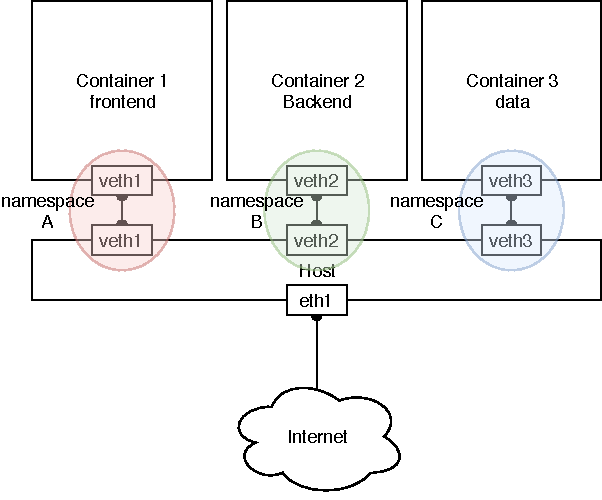
\includegraphics[width=0.9\textwidth]{bilder/network-topology.pdf}
		\caption{Netzwerk Topologie durch Trennung des Namespaces}
		\label{fig:containerHostNetwork}
	\end{center}
\end{figure} 


\subsection{Sicherheit}
\label{sec:sicherheit}

\begin{quote}
	\textit{"Docker is about running random code downloaded from the Internet and running it as root"}
	\flushright
	\small{---Dan Walsh (Red Hat)}
\end{quote}

Container haben ein großes Problem. Manche genannten Kernel-Features müssen als Nutzer \texttt{root} ausgeführt werden. Dadurch haben die gestarteten Prozesse häufig Berechtigungen, die es erlauben würden, aus der Isolierung des Containers auszubrechen. Um dies zu verhindern, können verschiedene Sicherheitskonzepte verwendet werden.

Das leichteste dieser Konzepte sind Capabilities. Jedem Prozess, sowie jeder Datei kann eine Liste an Capabilities zugeordnet oder genommen werden (siehe \fref{tab:capabilities}). Dabei können einzelnen Dateien beispielsweise die Rechte genommen werden, auf Port 80 zu hören. Auch viele Systemaufrufe können über Capabilites gewährt oder verwehrt werden.

Ein anderes Konzept ist die Implementation eines \textit{Mandatory Access Control}-Systems wie SELinux oder AppArmor. Diese Implementationen sind granularer als Capabilites, allerdings mit einem höheren Konfigurationsaufwand verbunden.

\begin{table}[h]
	\begin{center}
		\begin{tabu}to 0.9\textwidth{@{}lX[2,l]X[3,l]@{}}
			\toprule
			Capability 		& Systemaufruf 			& Erklärung						\\
			\midrule
			CAP\_CHOWN 		& chown 				& Ändern des Owners einer Datei \\
			CAP\_KILL 		& kill 					& Beenden eines Prozesses		\\
			CAP\_CHROOT		& chroot				& Wechseln des Root Directories	\\
			\midrule
			CAP\_NET\_BIND\_SERVICE & & Binden eines Prozesses auf Ports \textless 1024 \\
			\midrule
			CAP\_SYS\_TIME	& stime, settimeofday	& Setzen der Systemzeit 		\\
			CAP\_SYS\_ADMIN	& mount, umount, setns, pipe, syslog, ... 	& Alles, was in keine andere Kategorie passt 														\\
			\bottomrule
		\end{tabu}
	\end{center}
	\caption{Einige Capabilities \citep{Capabilities7LinuxManualPage}}
	\label{tab:capabilities}
\end{table}

\subsection{Container unter Windows}
\label{sec:windows}
Viele Kernel-Features des Linux-Kernels erlauben eine Isolation und wurden teilweise spezifisch für diese entwickelt \citep{Namespaces7LinuxManualPage}. Seit 2016 können spezifisch Docker-Container auch unter Windows genutzt werden. Dabei trennt Microsoft Container in zwei verschiedene Isolationen auf.

Windows Server Container 2016 sind ein nativer Windows Ansatz zur Isolation eines Prozesses. Dabei werden, wie bereits unter Linux Systemen, verschiedene Kernel-Technologien verwendet, um einen einzelnen Prozess zu isolieren. Der andere Ansatz sind Hyper-V Container. Diese nutzen minimale VM Instanzen zur Isolation eines Containers. Dabei ist der größte Unterschied, das Hyper-V Container eine minimale Instanz eines Windows Kernels nutzen, um auf diesem einzelne Isolationen zu erstellen, während Windows Server Container einen gemeinsamen Kernel nutzen.

\section{Eigene Implementierung}
\label{sec:eigeneImpl}
Um die in \fref{sec:funktionsweise} erläuterten Kernel-Features näher zu beleuchten wird folgend gezeigt, wie ein Prozess isoliert von einem Host-System ausgeführt werden kann. Dabei wird darauf eingegangen, wie ein tarball mit dem Tool buildroot erstellt werden kann. Dieser lässt sich folgend in Container-Runtimes wie rkt oder Docker importieren. Außerdem wird ein Prozess innerhalb des komprimierten Dateisystems mithilfe der Kernel-Funktionen aus \fref{sec:funktionsweise} isoliert. Das Ergebnis ist ein Dateisystem innerhalb eines Host-\gls{acr-os}, indem  eine Instanz der Python-Runtime isoliert und ohne Root-Berechtigungen ausgeführt wird.

\subsection{Erstellen eines tarballs}
\label{sec:tarball}
Bei einem tarball handelt es sich um ein komprimiertes Dateisystem. Buildroot ist ein Unix-Tool, welches zur Erstellung von minimalistischen Linux-Distributionen für Embedded-Systems entworfen wurde. Es erlaubt aber auch, nur ein Dateisystem zu erzeugen, ohne Kernel oder Init-System. Dies ist entscheidend, da bei Containern der bestehende Kernel des Host-OS mitbenutzt wird (\textit{siehe \fref{fig:containerVsVm}}). Ein Init-System wird in Containern nicht benötigt, da ihre Funktion das initialisieren neuer Prozesse ist. Container isolieren allerdings nur einen Prozess. Diese Features von buildroot erlauben es, einen tarball zu erzeugen, der als Dateisystem von Containern genutzt werden kann.

Zudem erlaubt es buildroot, einzelne Bibliotheken, wie zum Beispiel die Python-Runtime, beim Build-Prozess der Distribution zu integrieren. Nach dem Einstellen der benötigten Bibliotheken und dem Deaktivieren der für Container unnötigen Features erzeugt Buildroot ein Makefile. Durch das Starten des Build-Prozesses mit dem Befehl \texttt{make} wird die gewünschte Linux-Distribution erstellt. Am Ende dieses Prozesses liegt im Ordner /buildroot/out/images/ das gewünschte Dateisystem \texttt{rootfs.tar} (siehe \fref{fig:dirtreeNachBuildroot}).

\begin{figure}[h]
		\centering
		\begin{minipage}{0.9\textwidth}
			\dirtree{%
				.1 /home.
				.2 /buildroot.
				.3 /bin.
				.3 /out.
				.4 /images.
				.5 rootfs.tar.
			}
		\end{minipage}
		\caption{Dateisystem nach erfolgreichem Bauprozess mit buildroot}
		\label{fig:dirtreeNachBuildroot}
\end{figure} 


\subsection{Isolieren des tarballs}
\label{sec:isolieren}
In \fref{sec:tarball} wurde ein Dateisystem mit der Python-Runtime erstellt. Dieses muss nun isoliert, ein Pythonprogramm in das Dateisystem gemounted und ausgeführt werden.

Der erstellte tarball wird durch die in \fref{lst:untarRootfs} gezeigten \gls{gls-bash}-Befehle entpackt. Durch den Aufruf aus \fref{lst:untarRootfs} entsteht die in \fref{fig:baumNachUntar} zu sehende Dateistruktur.

\begin{listing}[h]
	\begin{minted}[breaklines]{bash}
cd /home
mkdir rootfs
cp rootfs.tar rootfs/
cd rootfs
sudo tar xvf rootfs.tar
sudo rm rootfs.tar
	\end{minted}
	\caption{Entpacken des buildroot tarballs nach /home/rootfs}
	\label{lst:untarRootfs}
\end{listing}


\begin{figure}[h]
	\centering
	\begin{minipage}{0.9\textwidth}
		\dirtree{%
			.1 /home/rootfs/.
			.2 usr.
			.3 bin.
			.4 python -> python3.6.\DTcomment{nicht aus Hostsystem}.
			.4 python3.6.
		}
	\end{minipage}
	\caption{Dateibaum nach entpacken der \texttt{rootfs.tar}}
	\label{fig:baumNachUntar}
\end{figure}

Um einen Prozess mit dem Wurzelverzeichnis \texttt{/home/rootfs/} auszuführen, ist lediglich der Aufruf \mintinline{bash}{sudo chroot rootfs /usr/bin/python3.6 -m http.server} nötig.

Durch diesen wird ein Webserver auf Adresse \texttt{http://0.0.0.0:8000} ausgeführt, der alle ihm zugänglichen Dateien zum Download bereitstellt. Beim Aufrufen dieser Adresse erkennt man, dass der Webserver nur Zugriff auf die in \texttt{/home/rootfs/} liegenden Dateien hat, wie in \fref{fig:chrootPythonWebserver} gezeigt.

\begin{figure}[H]
	\begin{center}
		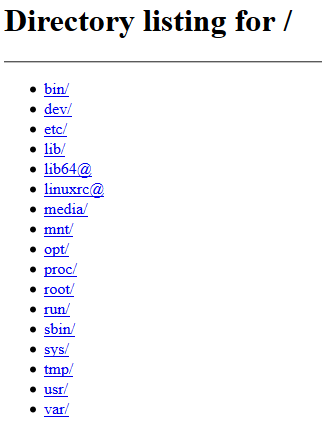
\includegraphics[scale=0.7]{bilder/chroot-python-webserver.png}
		\caption{Python Webserver mit festgesetztem Root-Verzeichnis}
		\label{fig:chrootPythonWebserver}
	\end{center}
\end{figure}

Um weiterhin Zugriff auf dynamische Inhalte aus dem Host-System zu haben, kann man, wie in \fref{sec:mount} erklärt, entsprechende Verzeichnisse in das neue rootfs des Prozesses mounten (siehe \fref{lst:mountReadOnly}).

\begin{listing}[h]
	\begin{minted}[breaklines]{bash}
nsenter --mount=/proc/<PID isolierter Prozess>/ns/mnt \
mount --bind -o ro $PWD/readonly $PWD/rootfs/var/src
	\end{minted}
	\caption{Mounten von Verzeichnis \texttt{/readonly/} zu \texttt{/rootfs/var/src/}}
	\label{lst:mountReadOnly}
\end{listing}

Durch die Dateitrennung und den Aufruf von \texttt{chroot} tritt allerdings ein großes Problem auf. Der Python-Webserver wird mit erhöhten Rechten ausgeführt, da diese für den Aufruf von \texttt{chroot} benötigt werden (siehe \fref{fig:chrootWhoami}).

\begin{figure}[h]
	\begin{center}
		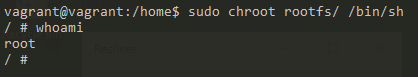
\includegraphics[scale=1]{bilder/chroot-whoami-root.png}
		\caption{Root-Eskalation durch Aufruf von \texttt{sudo chroot}}
		\label{fig:chrootWhoami}
	\end{center}
\end{figure}

Dies führt zu vielen Problemen. Ein Prozess, der nur auf diese Weise isoliert wird, könnte beispielsweise Prozesse auf dem Hostsystem mit \texttt{kill <pid>} beenden. Die Lösung dieses Problems sind die in \fref{sec:namespaces} beschriebenen namespaces.

Um alle Prozesse des Hostsystems vor dem Container zu verstecken, muss der PID-Namespace des Container-Prozesses neu gemounted werden, wie in \fref{lst:unshareRemount} beschrieben.
\begin{listing}[h]
	\begin{minted}[breaklines, breakafter=/]{bash}
sudo unshare -p --mount-proc=$PWD/rootfs/proc -f chroot rootfs /bin/sh
	\end{minted}
	\caption{Remount des PID-Namespaces und Chroot einer Shell}
	\label{lst:unshareRemount}
\end{listing}

Beim Aufruf von \glqq \mintinline{bash}{ps aux}\grqq{} wird nur noch der Prozess \texttt{/bin/sh} angezeigt, der die PID 1 bekommen hat. Dieses Vorgehen löst allerdings nicht die Ursache des Problems. Der gestartete Prozess läuft auch weiterhin unter dem Nutzer root. Ein auf diese Weise isolierter Prozess kann zum Beispiel auf Port 80 hören. Um diese Berechtigungen zu entfernen werden die in \fref{sec:sicherheit} angesprochenen Capabilites verwendet.

Durch den Aufruf von \mintinline[breaklines]{bash}{capsh --drop=cap_net_bind_service --chroot=root fs/ --} hat die in rootfs gestartete \texttt{/bin/bash} nicht mehr die Möglichkeit, auf niedrigere Ports wie Port 80 zu hören.


Um vollständige Isolation des Containers zu erreichen, müssen Systemressourcen, wie Arbeitsspeicher oder CPU-Zyklen, limitiert werden. Dazu dienen die in \fref{sec:cgroups} beschriebenen \glspl{acr-cgroup}.

Um eine \gls{acr-cgroup} zu erstellen, muss ein Ordner unterhalb der cgroup Dateihierarchie erstellt werden. Folgend kann man einen Prozess einer \gls{acr-cgroup} zuweisen, indem man die PID des Prozesses in die Datei \texttt{/sys/fs/cgroup/CONTROLLER/} \texttt{CGROUPNAME/tasks} schreibt (siehe \fref{lst:cgroupZuweisen}).

\begin{listing}[h]
	\begin{minted}[breaklines, breakafter=/]{bash}
mkdir /sys/fs/cgroup/memory/container
echo $ContainerPID > /sys/fs/cgroup/memory/container/tasks
	\end{minted}
	\caption{Erzeugen einer memory cgroup namens container}
	\label{lst:cgroupZuweisen}
\end{listing}

CGroups dienen dazu, Systemressourcen zu limitieren. Dazu können Limits in entsprechende Pseudo-Filehandles geschrieben werden. Um z.B. die Arbeitsspeichermenge auf \tildeawesome100Mb zu limitieren, können die in \fref{lst:limitRam} gezeigten Bash-Befehle ausgeführt werden. 

\begin{listing}[h]
	\begin{minted}[breaklines, breakafter=/]{bash}
echo "0" > /sys/fs/cgroup/memory/container/memory.swappiness
echo "100000000" > /sys/fs/cgroup/memory/container/memory.limit_in_bytes
	\end{minted}
	\caption{Limitieren des Arbeitsspeichers und Memory-Swap deaktivieren}
	\label{lst:limitRam}
\end{listing}

Um zu testen, ob die Zuweisung funktioniert und durch den isolierten Prozess maximal \tildeawesome100Mb Arbeitsspeicher belegt werden können, kann das Python Programm aus \fref{lst:hungry-py} ausgeführt werden. \fref{fig:cgroupKilled} zeigt die Ausgabe des Prozesses, der sich in der \gls{acr-cgroup} container befindet.

\begin{listing}[hp]
	\begin{minted}[]{python}
#hungry.py - Eating up memory in 10Mb blocks
import time

TEN_MEGABYTE = 10000000

f = open("/dev/urandom", "rb")
data = bytearray()
i = 0

while True:
	data.extend(f.read(TEN_MEGABYTE))
	i += 1
	print("%dMb belegt" % (i*10,))
	time.sleep(1)
	\end{minted}
	\caption{Python Programm hungry.py um Arbeitsspeicher zu verbrauchen}
	\label{lst:hungry-py}
\end{listing}


\begin{figure}[hp]
	 \begin{center}
	 	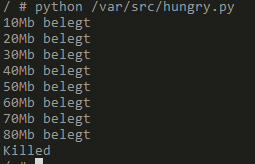
\includegraphics[scale=1.3]{bilder/cgroup-container-killed.png}
	 	\caption{Ausgabe des Pythonprogramms \texttt{hungry.py}}
	 	\label{fig:cgroupKilled}
	 \end{center}
\end{figure}

\subsubsection{Fazit}
\label{sec:eigImplFazit}

Durch das beschriebene Vorgehen kann ein beliebiger Prozess auch ohne Con"-tai"-ner-Run"-time isoliert werden. Diese simplifizieren das Vorgehen aber erheblich. So kann mit Ergebnis das selbe Verhalten durch die Commandozeile \texttt{docker run -d python:alpine3.6} erreicht werden